\section{Bernie Stone Case Study}\label{sec:case_study}
This section discusses the Bernie Stone case study, which is the primary motivation for this paper.
Bernie Stone was an alderman in Chicago's 50th ward from 1973 to 2011.
He was well known for his, ``political philosophy.''

\begin{quotation}
    ``You take care of the people who take care of you — you know, the people who voted for you, That’s not Chicago politics, that’s Politics 101.'' - Alderman Bernie Stone (50th ward), Quoted from~\cite{BGA_berniequote}
\end{quotation}

In fact an alderman who grew up in the 50th ward once remarked that,

\begin{quotation}
    ``Well, I grew up in the 50th Ward and you know, God bless [the late former Ald.] Bernie Stone, may he rest in peace, but I remember crossing California going west, every street was resurfaced almost every year. They always had brand new lighting and then east of California, where he would lose the precincts consistently, I mean the streets were in shambles. Many people felt he was spending the bulk of the menu money west of California, where he was getting the bulk of the vote.'' - Alderman Carlos Ramirez-Rosa (35th Ward), Quoted from~\cite{ramirezrosaquote}
\end{quotation}

This quote is a clear example of the type of behavior that this paper seeks to investigate.
This phenomena could not be verified previously because the CDOT did not make the documents publicly available. 
Furthermore, the data that did exist, was in PDF form, making locating the spending tedious and difficult.
Thus this paper is the first to put numbers to this anecdotal evidence.
First we can look at a map of the precincts that supported Stone financially and electorally.
Below in Figure~\ref{fig:stone_support_maps} we can see the precincts that supported Stone in the 2007 runoff election and the precincts that gave Stone the most individual contributions.
In both maps we can clearly see that the south western portion of the ward is the most supportive of Stone, on average.
\begin{figure}[H]
    \centering
    % First subfigure
    \begin{subfigure}[b]{0.45\textwidth} % [b] aligns at the bottom
    \includegraphics[width=\textwidth]{input/contribution_map_stone_ward_50_2003_2011.png}
    \caption{Campaign contributions to Alderman Stone, 2003-2011}
    \end{subfigure}
    \hfill % This adds some space between the two subfigures
    % Second subfigure
    \begin{subfigure}[b]{0.45\textwidth}
    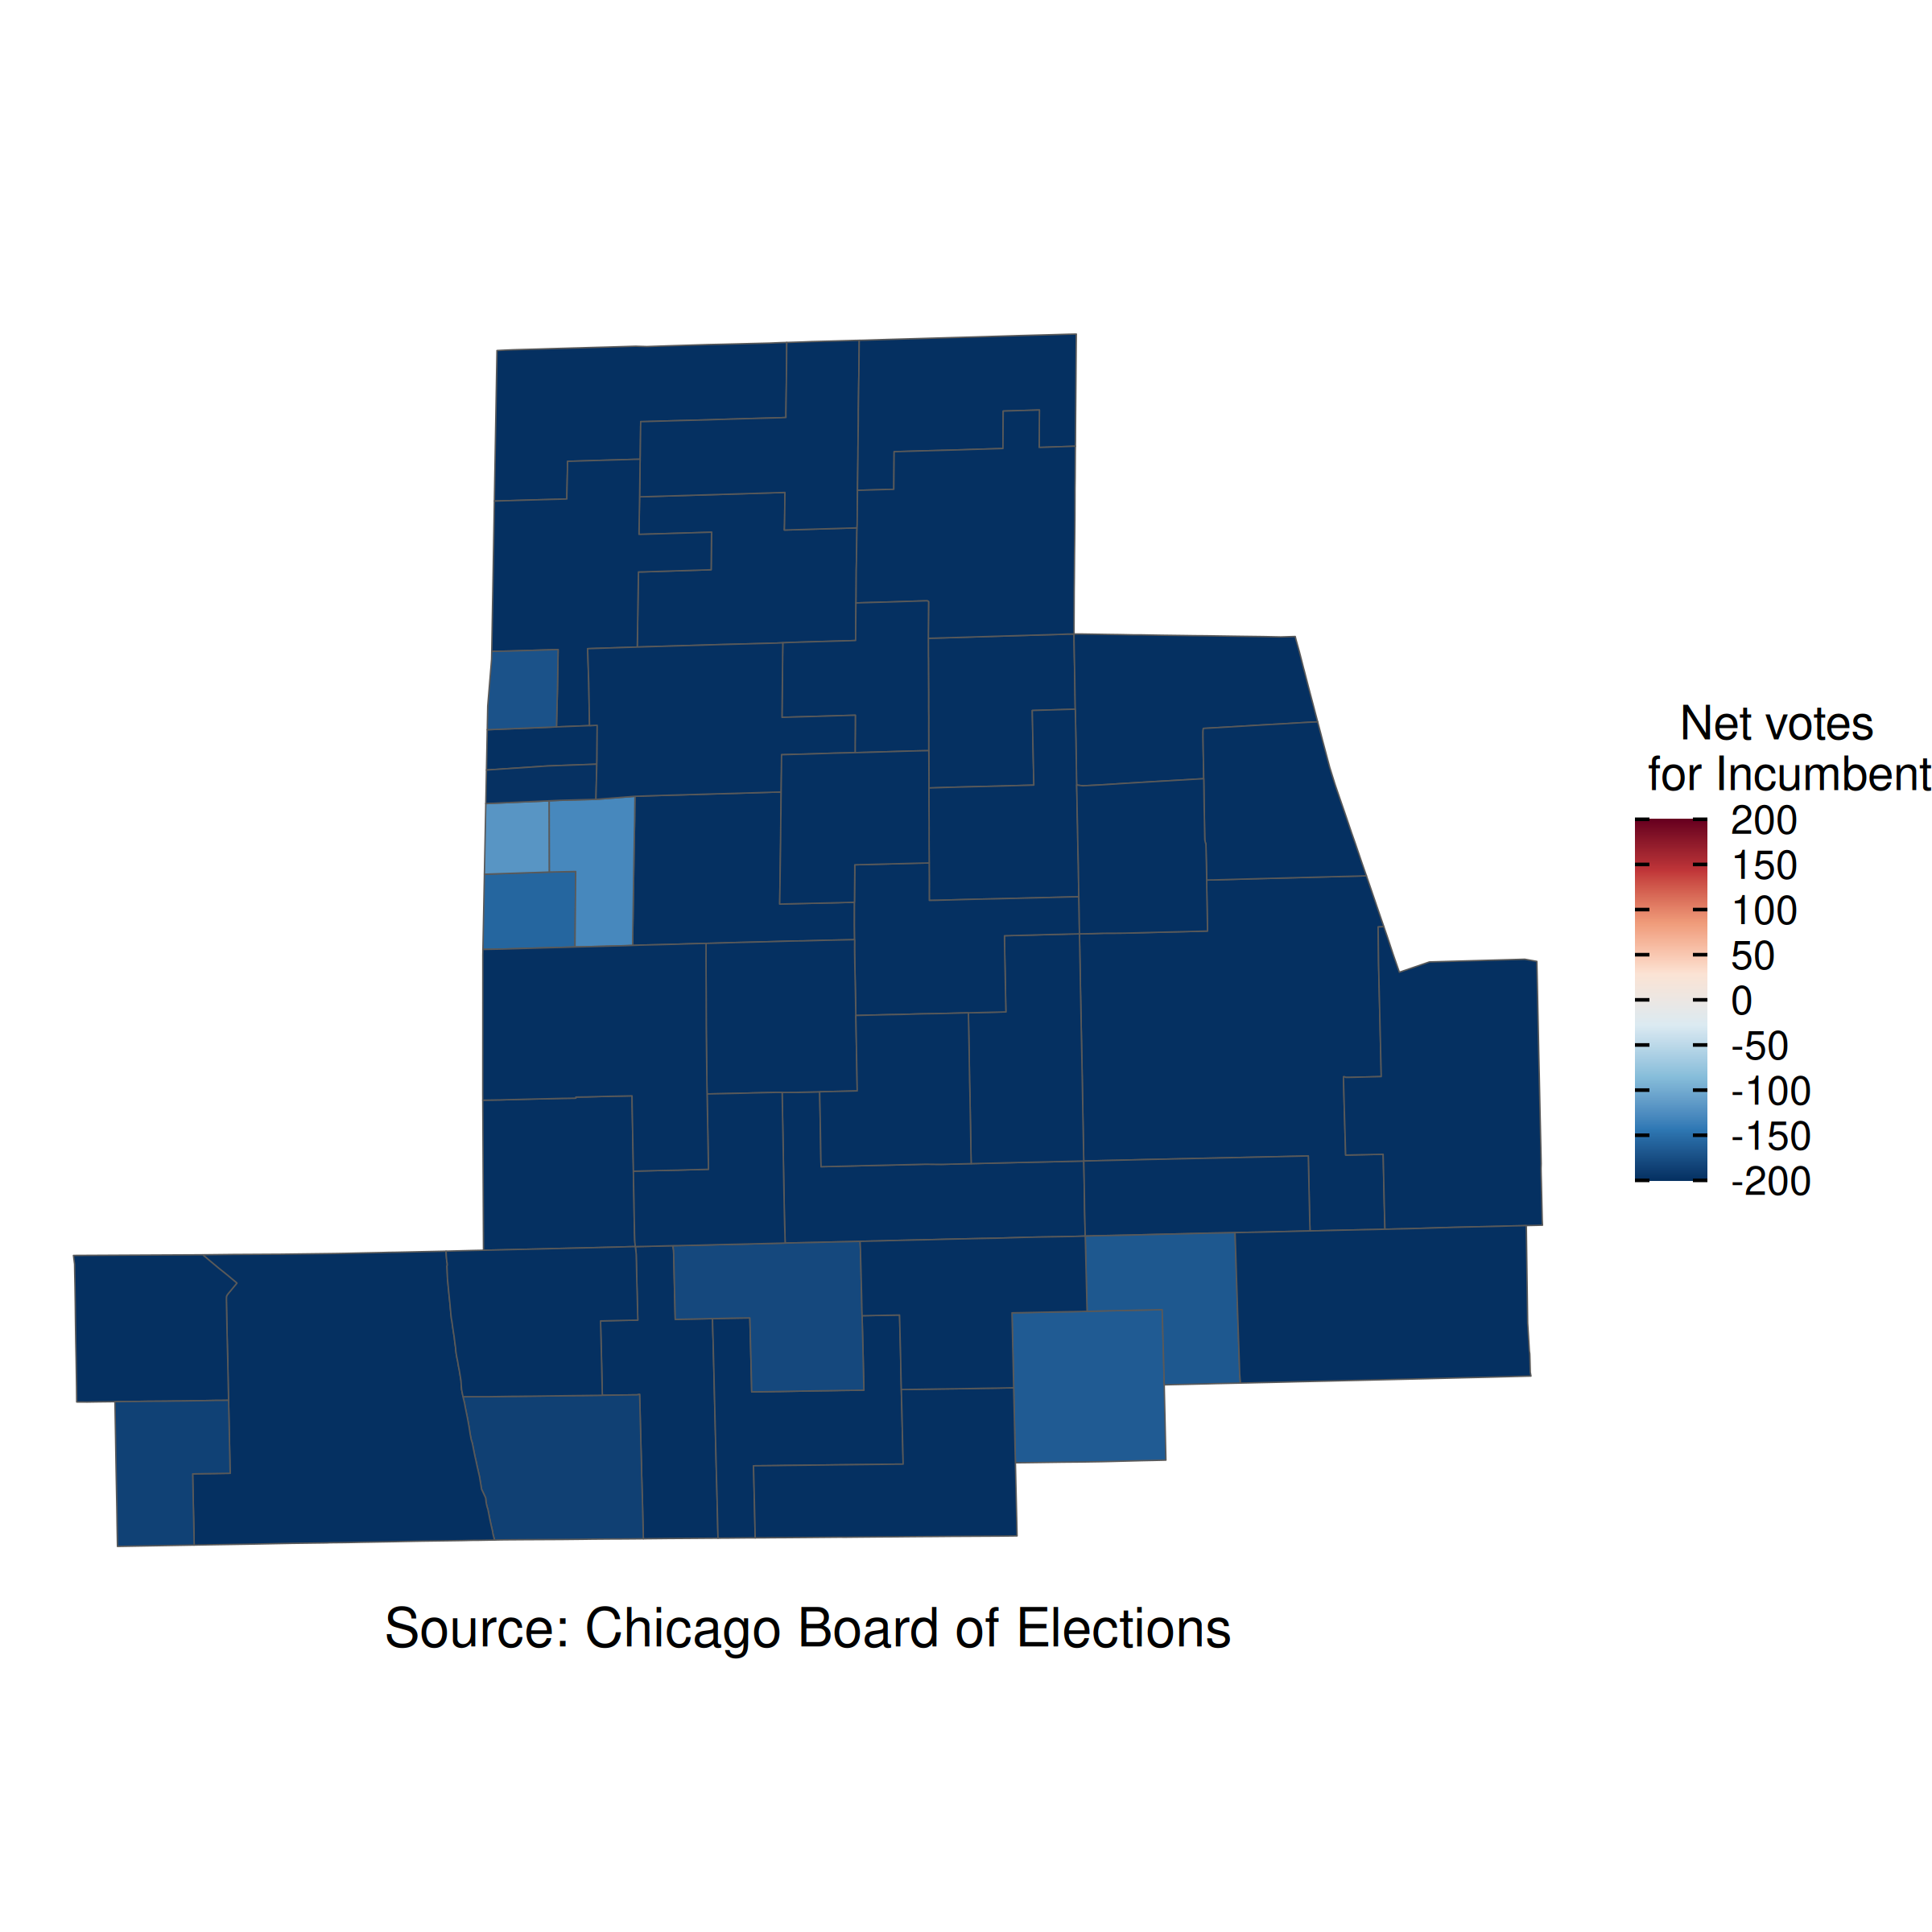
\includegraphics[width=\textwidth]{input/ward_50_2007_runoff_incumbent_precinct_results.png}
    \caption{Net votes for Alderman Stone, 2007}
    \end{subfigure}
    \caption{Distribution of Spending per Precinct for both ward maps in the dataset}
    \label{fig:stone_support_maps}
\end{figure}

Next, we can look at a time series of the spending per precinct for the 50th ward. 
There are approximately 44 precincts in the 50th ward, so Figure~\ref{fig:stone_spending_timeline} gathers the top and bottom quintile of precincts by contributions to Stone and shows average fraction of the total located budget spent in each quintile. 
``other'' refers to all other precincts.
Note, that the precincts that contributed the most to Stone's campaign are the same precincts that contributed the most net votes to Stone in the 2007 runoff election.
We see that after his reelection in 2007, Stone's spending per precinct is heavily concentrated in the precincts that supported him.
After his defeat, spending per precinct is much more evenly distributed across the ward.

\begin{figure}[H]
    \centering
    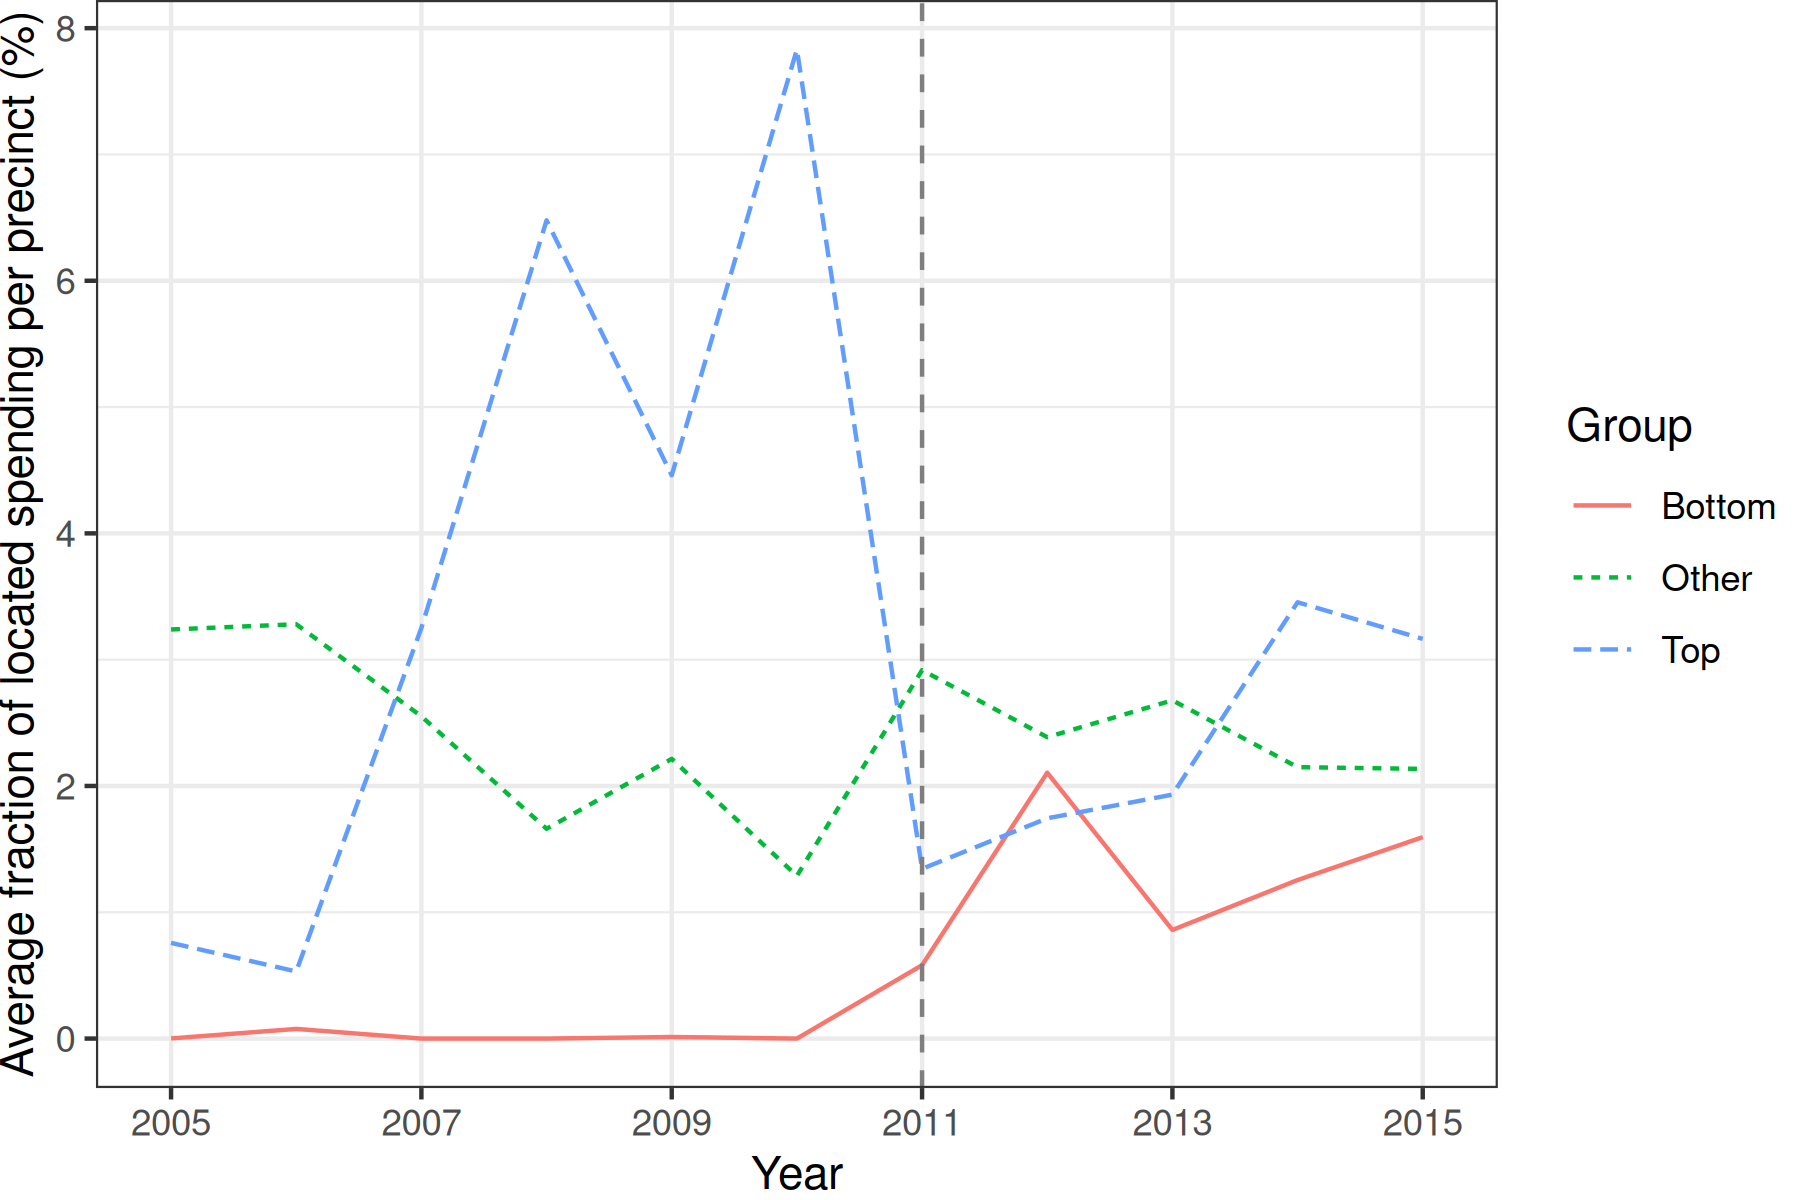
\includegraphics[width=0.8\textwidth]{input/ward_50_contribution_8_precincts_timeline.png}
    \caption{Average Spending per Precinct in the 50th Ward, 2005-2016}
    \label{fig:stone_spending_timeline}
\end{figure}

Finally, we can look at the 50th ward's spending per precinct in the years leading up to and following Stone's defeat in 2011 via a map in Figure~\ref{fig:stone_spending_maps}.
This shows a clear shift in spending from the south-western portion of the ward, to a roughly even distribution across the ward.

\begin{figure}[H]
    \centering
    % First subfigure
    \begin{subfigure}[b]{0.45\textwidth} % [b] aligns at the bottom
    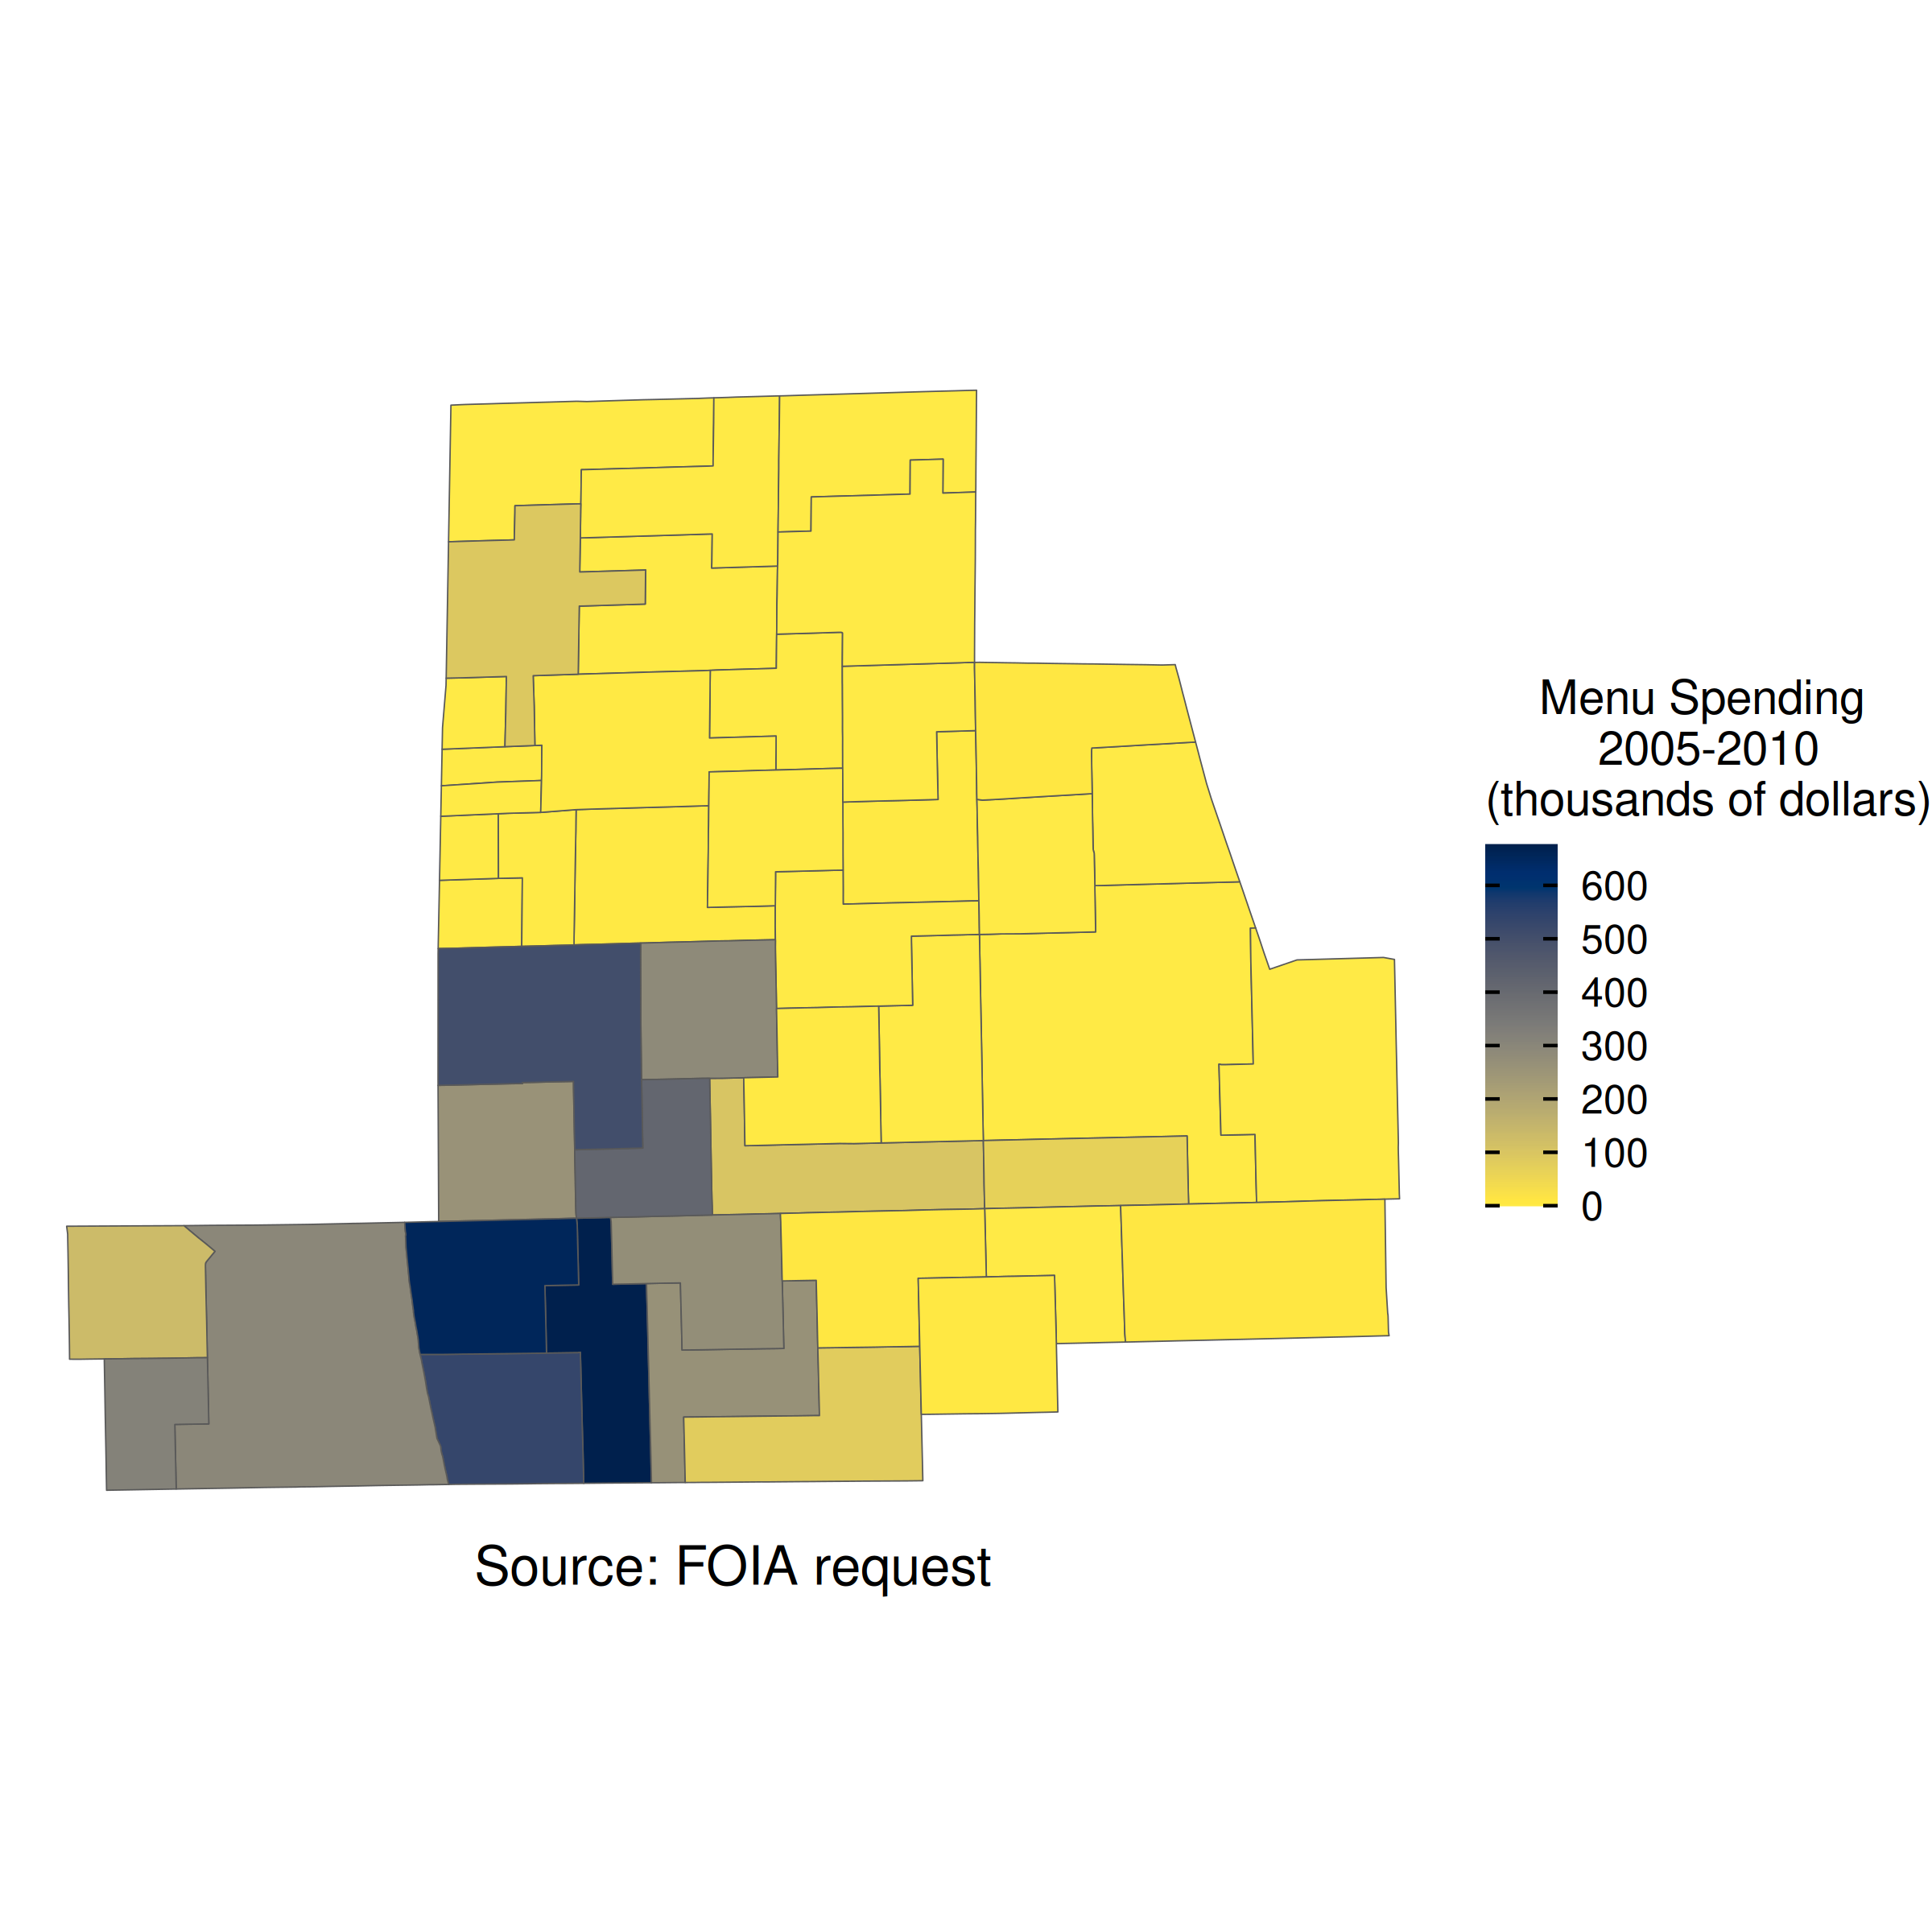
\includegraphics[width=\textwidth]{input/ward_50_menu_map_2005_2010.png}
    \caption{50th Ward Menu Allocation, 2005-2010}
    \end{subfigure}
    \hfill % This adds some space between the two subfigures
    % Second subfigure
    \begin{subfigure}[b]{0.45\textwidth}
    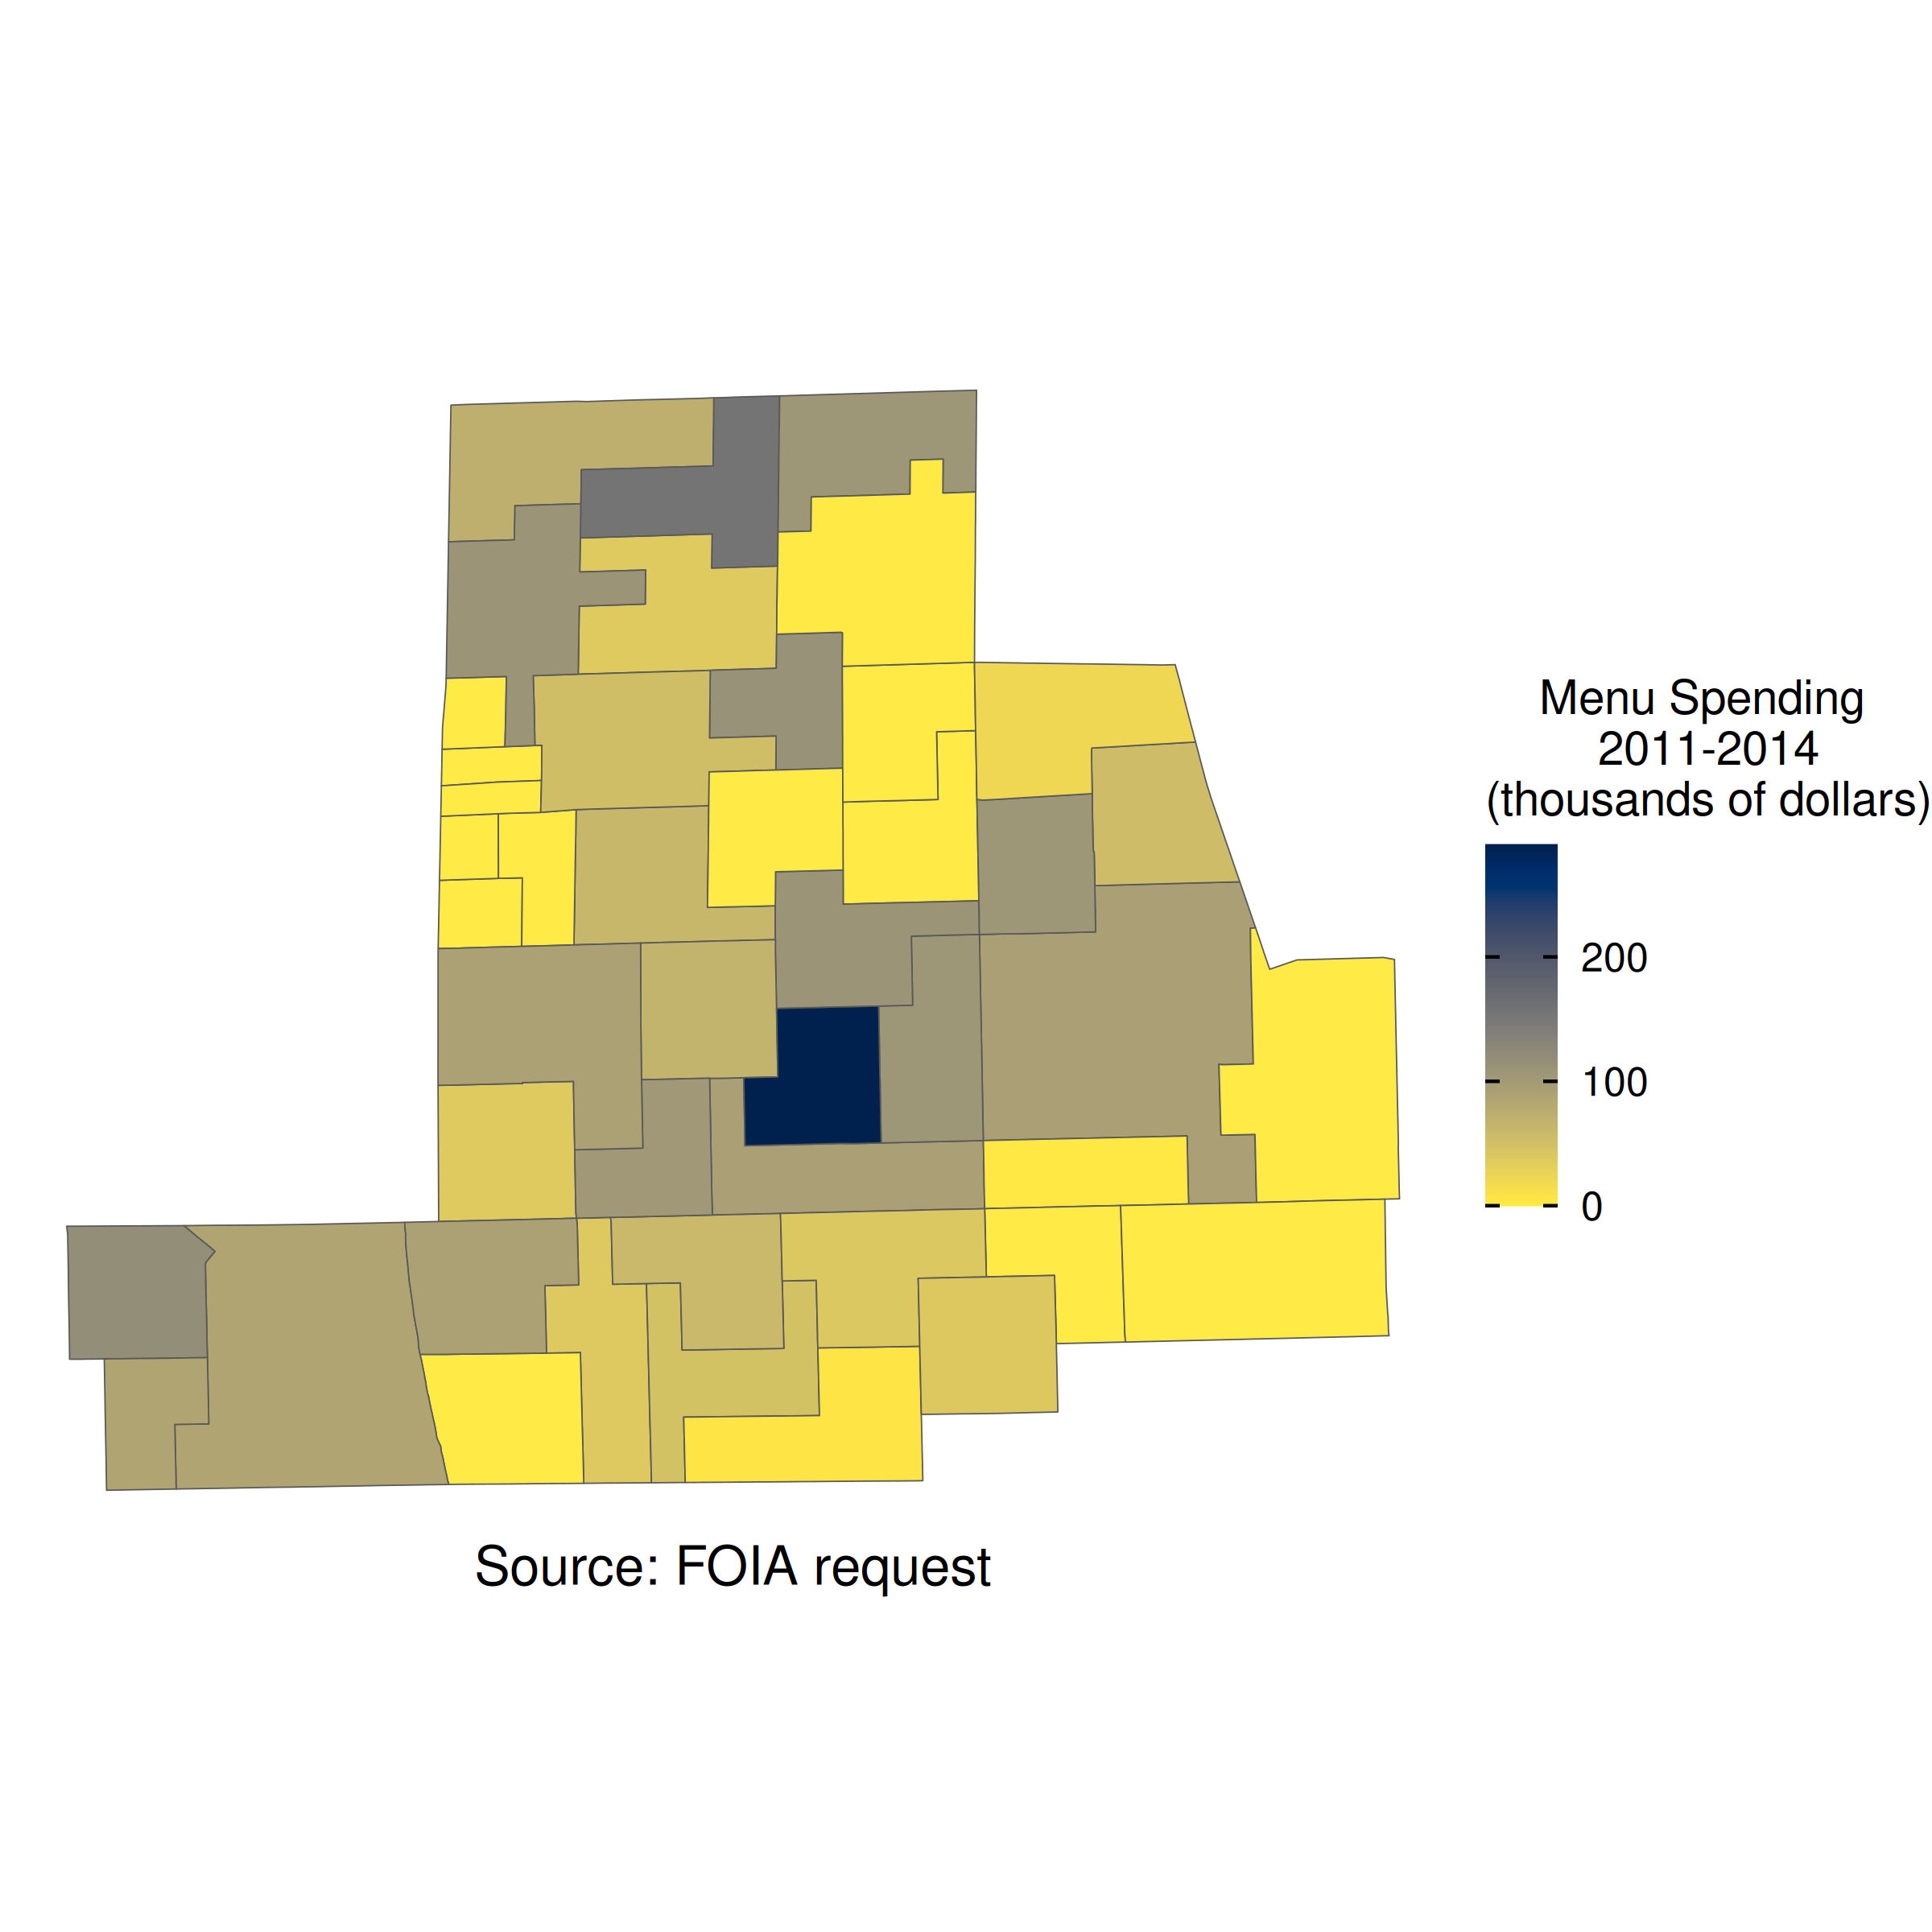
\includegraphics[width=\textwidth]{input/ward_50_menu_map_2011_2014.png}
    \caption{50th Ward Menu Allocation, 2011-2015}
    \end{subfigure}
    \caption{50th Ward Menu Allocation, 2011-2016}
    \label{fig:stone_support_maps}
\end{figure}

